% Copyright (c) 2018 Victorien Elvinger
% Code licensed under GPLv3 (https://www.gnu.org/licenses/gpl-3.0.en.html).
% Content licensed under CC-BY 4.0 (https://creativecommons.org/licenses/by/4.0/).

\documentclass[xcolor=table]{beamer}
\usetheme{metropolis}

\usepackage[utf8]{inputenc}
\usepackage{amsmath}
\usepackage{hyperref}
\usepackage{acronym} % \ac[p], \acl[p], \acs[p], \acf[p]

\usepackage[scale=1.5]{ccicons}

\usepackage{color}
\usepackage{tikz}
\usetikzlibrary{arrows,arrows.meta,calc,positioning}

\usepackage{transparent}

\graphicspath{{./fig/}}

\usepackage{silence}
\WarningFilter{biblatex}{Patching footnotes failed}
    % Filter warning of biblatex package: "Patching footnotes failed"

\usepackage[backend=biber,defernumbers=true,style=trad-plain,sorting=ydnt,maxbibnames=1,maxcitenames=1]{biblatex}
\addbibresource{references.bib}
\AtBeginBibliography{\footnotesize}
\setbeamertemplate{bibliography item}[text] % use ref number in bibliography

\renewcommand{\thefootnote}{[\arabic{footnote}]}


% Colors
% ------
% Prefix every color with 'uc' (user-defined color)

\definecolor{uctrusted}{HTML}{00CC00}

% Tikz styles
% -----------
\tikzset{com/.style = {dotted,line width=1.2pt}}
\tikzset{unicast/.style = {com,->,> = latex'}}
\tikzset{trusted/.style = {draw,shape=rectangle,fill=white,minimum size=1.6em}}
\tikzset{username/.style = {text width={width("mallory ")},align=right}}

\tikzset{timeline/.style = {->,> = latex'}}

\tikzset{event/.style = {draw,shape=circle,fill=white,text width={width ("AA")},align=center}}
%\tikzset{trusted/.style = {shape=rectangle}}

\tikzset{ulabel/.style = {draw,shape=rectangle,fill=white,minimum width=2.2em,minimum height=1.1em}}

\tikzset{precedes/.style = {->,line width=1pt,> = latex'}}

% User-defined commands
% ---------------------
% Prefix every command with 'u' (u like user)

\newcommand{\ufcounter}[1]{
    % 1: maximum count
    \foreach[count=\counter] \i in {1, ..., #1} {\only<\i|handeout:0>{\i}}
}

\newcommand{\ufcircledcounter}[2]{
    % 1: position, 2: maximum count
    \node[fill,circle] (fcount) at (#1) {};
    \node[text=white,font=\scriptsize] at (fcount) {\ufcounter{#2}};
}

\newenvironment{utikzhbgraph}{%
    %% \uevent{node-id}{position}{content}
    \newcommand{\uevent}[3]{\node[event] (##1) at (##2) {};\node[] at (##1) {##3};}%
    %% \upre{source}{target}
    \newcommand{\uhb}[2]{\draw[precedes] (##1) to (##2);}%
    %% \ulabelled{labelled-node-id}{at-most-five-letter-label}
    \newcommand{\ulabelled}[2]{\node[ulabel,below left=-1pt and -4pt of ##1] (l##1) {};\node[] at (l##1) {##2};}%
    %% \uembedded{embedded-node-id}{relative-pos}{text}
    %% relative-pos: below|above left|right
    \newcommand{\uembedded}[3]{%
        \node[##2=-7.5pt and -7.5pt of ##1] (uembeddedp0##1) {};%
        \node[##2=10pt and 1pt of ##1] (uembeddedp1##1) {};%
        \draw[-Circle] (uembeddedp1##1) to (uembeddedp0##1);%
        \node[##2=-10pt and -7pt of uembeddedp1##1] {##3};}%
    %% \uparticipants{event-node-id}{relative-pos}{coma-seperated-list-of-participants}
    %% relative-pos: below|above left|right
    \newcommand{\uparticipants}[3]{\uembedded{##1}{##2}{$\left\{##3\right\}$}}%
    \begin{tikzpicture}%
}{%
    \end{tikzpicture}%
}

% Acronyms
% --------
\acrodef{FJC}[FJC]{Fork-Join-Causal}
\acrodef{VFJC}[VFJC]{View-\acl{FJC}}

% Meta-data
% ---------

\author{Victorien Elvinger}
\title{Prunable Authenticated Log\\ and Authenticable Snapshot\\ in Distributed Collaborative Systems}
\institute{%
    
\includegraphics[height=1.6em]{/logo/loria.pdf}\hspace{1.6em}%
    
\includegraphics[height=1.6em]{/logo/ul.pdf}\hspace{1.6em}%
    
\includegraphics[height=1.6em]{/logo/cnrs.pdf}\hspace{1.6em}%
    
\includegraphics[height=1.6em]{/logo/inria.pdf}\hspace{1.6em}%
    \newline Supervised by Gérald Oster and François Charoy%
}
\date{October 2018}

% Content
% -------

\begin{document}

\maketitle

\begin{frame}{Peer-to-Peer Collaborative Systems}
    \begin{figure}\begin{tikzpicture}
        \node at (-3.5,0) {}; % Animation fix
        \node at (5.5,0) {}; % Animation fix
        \ufcircledcounter{-2.8, 2.1}{6} % Animation frame count

        % Participants and documents
        \node[label=below:{\textbf{A}lice}] (A) at (0, 0) {
            
\includegraphics[scale=0.4]{materials/device.pdf}};
        \node[left=1pt of A,minimum height=4] (docA) {
            \includegraphics<1-3 | handout:0>[scale=0.4]{materials/doc-a1.pdf}
            \includegraphics<4,5 | handout:0>[scale=0.4]{materials/doc-a2.pdf}
            \includegraphics<6>[scale=0.4]{materials/doc-a2-b1.pdf}
        };
        \node[left=-3pt of docA] {
            \only<1 | handout:0>{$a_1($
\includegraphics[scale=0.4]{materials/doc.pdf}$) =$}%
            \only<4 | handout:0>{$a_2($
\includegraphics[scale=0.4]{materials/doc-a1.pdf}$) =$}%
            \only<6>{$b_1($
\includegraphics[scale=0.4]{materials/doc-a2.pdf}$) =$}
        };

        \node[label=above:{\textbf{B}ob}] (B) at (2.1, 1.4) {
            
\includegraphics[scale=0.4]{materials/device.pdf}};
        \node[above right=-22pt and 1pt of B] (docB) {
            \includegraphics<3 | handout:0>[scale=0.4]{materials/doc-a1.pdf}
            \includegraphics<4,5 | handout:0>[scale=0.4]{materials/doc-a1-b1.pdf}
            \includegraphics<6>[scale=0.4]{materials/doc-a2-b1.pdf}
        };
        \node[right=-3pt of docB] {
            \only<4 | handout:0>{$= b_1($
\includegraphics[scale=0.4]{materials/doc-a1.pdf}$)$}%
            \only<6>{$= a_2($
\includegraphics[scale=0.4]{materials/doc-a1-b1.pdf}$)$}
        };

        \node[label=below:{\textbf{M}allory}] (C) at (2.2, -0.5) {
            
\includegraphics[scale=0.4]{materials/device.pdf}};
        \node[right=1pt of C] {
            \includegraphics<3-5 | handout:0>[scale=0.4]{materials/doc-a1.pdf}
            \includegraphics<6>[scale=0.4]{materials/doc-a2-b1.pdf}
        };

        % Network and packets
        \draw<1,3,4,6>[com] (A) to (B);
        \draw<2 | handout:0>[unicast] (A) -- (B) node[near start] {
            
\includegraphics[scale=0.4]{materials/contrib-a1.pdf}};
        \draw<5>[com] (A) -- (B) node[midway] {
            
\includegraphics[scale=0.4]{materials/sync.pdf}};

        \draw<1,3,4,6>[com] (A) to (C);
        \draw<2 | handout:0>[unicast] (A) -- (C) node[near start] {
            
\includegraphics[scale=0.4]{materials/contrib-a1.pdf}};
        \draw<5>[com] (A) -- (C) node[midway] {
            
\includegraphics[scale=0.4]{materials/sync.pdf}};

        \draw<1-4,6>[com] (B) to (C);
        \draw<5 | handout:0>[com] (B) -- (C) node[midway] {
            
\includegraphics[scale=0.4]{materials/sync.pdf}};
    \end{tikzpicture}\end{figure}
    \begin{itemize}
        \item participants issue \textbf{operations} to update a shared document
        \item<3-> participants have their \textbf{own copy} of \textbf{co-authored data}
        \begin{itemize}
            \item<4-> \textbf{always-available}
            \item<4-> continuously \textbf{diverge then converge} from others
            \item<6-> convergence as a \textbf{liveness property}
        \end{itemize}
    \end{itemize}
    \vspace{1em} % layout fix
\end{frame}

\begin{frame}{Threat to convergence}
    \begin{figure}\begin{tikzpicture}
        \node at (-3.5,0) {}; % Animation fix
        \node at (5.5,0) {}; % Animation fix
        \ufcircledcounter{-1.1, 2.1}{5} % Animation frame count

        % Participants and documents
        \node[label=below:{\textbf{A}lice}] (A) at (0, 0) {
            
\includegraphics[scale=0.4]{materials/device.pdf}};
        \node[left=1pt of A] (docA) {
            \includegraphics<1 | handout:0>[scale=0.4]{materials/doc-a3-b1.pdf}
            \includegraphics<2 | handout:0>[scale=0.4]{materials/doc-a3-b1-m1p.pdf}
            \includegraphics<3,4 | handout:0>[scale=0.4]{materials/doc-a4-b1-m1p.pdf}
            \includegraphics<5>[scale=0.4]{materials/doc-a4-b2-m1p.pdf}
        };
        \node[left=-3pt of docA] {
            \only<2 | handout:0>{$m_1'($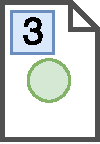
\includegraphics[scale=0.4]{materials/doc-a3-b1.pdf}$) =$}%
            \only<3 | handout:0>{$a_4($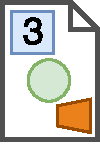
\includegraphics[scale=0.4]{materials/doc-a3-b1-m1p.pdf}$) =$}%
            \only<5>{$b_2($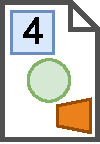
\includegraphics[scale=0.4]{materials/doc-a4-b1-m1p.pdf}$) =$}%
        };

        \node[label=above:{\textbf{B}ob}] (B) at (2.1, 1.4) {
            
\includegraphics[scale=0.4]{materials/device.pdf}};
        \node[above right=-22pt and 1pt of B] (docB) {
            \includegraphics<1 | handout:0>[scale=0.4]{materials/doc-a3-b1.pdf}
            \includegraphics<2 | handout:0>[scale=0.4]{materials/doc-a3-b1-m1.pdf}
            \includegraphics<3,4 | handout:0>[scale=0.4]{materials/doc-a3-b2-m1.pdf}
            \includegraphics<5>[scale=0.4]{materials/doc-a4-b2-m1.pdf}
        };
        \node[right=-3pt of docB] {
            \only<2 | handout:0>{$= m_1($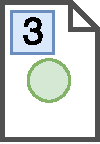
\includegraphics[scale=0.4]{materials/doc-a3-b1.pdf}$)$}%
            \only<3 | handout:0>{$= b_2($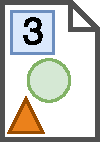
\includegraphics[scale=0.4]{materials/doc-a3-b1-m1.pdf}$)$}%
            \only<5>{$= a_4($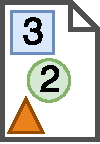
\includegraphics[scale=0.4]{materials/doc-a3-b2-m1.pdf}$)$}%
        };

        \node[label=below:{\textbf{M}allory}] (M) at (2.2, -0.5) {
            
\includegraphics[scale=0.4]{materials/device-malicious.pdf}};

        % Network and packets
        \draw<1-3,5>[com] (A) to (B);
        \draw<4>[com] (A) -- (B) node[midway] {
            
\includegraphics[scale=0.4]{materials/sync.pdf}};

        \draw<2->[com] (M) to (A);
        \draw<1 | handout:0>[unicast] (M) -- (A) node[near start] {
            
\includegraphics[scale=0.4]{materials/contrib-m1p.pdf}};

        \draw<2->[com] (M) to (B);
        \draw<1 | handout:0>[unicast] (M) -- (B) node[near start] {
            
\includegraphics[scale=0.4]{materials/contrib-m1.pdf}};
    \end{tikzpicture}\end{figure}
    \begin{itemize}
        \item Byzantine\footfullcite{lamport_byzantine_1982} adversary
        \begin{itemize}
            \item \textbf{colluding malicious participants + network}
            \item can \textbf{conceal divergences} using \textbf{equivocation}
        \end{itemize}
        \item unlimited exchanges between honest participants
    \end{itemize}
    \vspace{1em}
\end{frame}

\begin{frame}{Authenticated logs}
    \begin{columns}
        \begin{column}{0.25\textwidth}
            \begin{figure}\begin{utikzhbgraph}
                \node at (-1,0) {}; % Animation fix

                \node (prefix) at (0, 0) {$\ldots$};

                \uevent{a3}{0,-1}{$a_3$}
                \uhb{prefix}{a3}

                \uevent{m1p}{0.7,-2}{$m_1'$}
                \uevent{a4}{0.7,-3.1}{$a_4$}
                \uhb{a3}{m1p})
                \uhb{m1p}{a4};

                \only<2> {
                    \uevent{m1}{-0.7,-2}{$m_1$}
                    \uevent{b2}{-0.7,-3.1}{$b_2$}

                    \uhb{a3}{m1}
                    \uhb{m1}{b2}
                }
            \end{utikzhbgraph}\end{figure}
        \end{column}
        \begin{column}{0.5\textwidth}
            \begin{figure}\begin{tikzpicture}
                \ufcircledcounter{-1.1, 2.1}{2} % Animation frame count

                % Participants and documents
                \node[label=below:{\textbf{A}lice}] (A) at (0, 0) {
                    
\includegraphics[scale=0.4]{materials/device.pdf}};
                \node[left=1pt of A] {
                    \includegraphics<1 | handout:0>[scale=0.4]{materials/doc-a4-b1-m1p.pdf}
                    \includegraphics<2>[scale=0.4]{materials/doc-a4-b2-m1-m1p.pdf}
                };

                \node[label=above:{\textbf{B}ob}] (B) at (2.1, 1.4) {
                    
\includegraphics[scale=0.4]{materials/device.pdf}};
                \node[above right=-22pt and 1pt of B] {
                    \includegraphics<1 | handout:0>[scale=0.4]{materials/doc-a3-b2-m1.pdf}
                    \includegraphics<2>[scale=0.4]{materials/doc-a4-b2-m1-m1p.pdf}
                };

                \node[label=below:{\textbf{M}allory}] (M) at (2.2, -0.5) {
                    
\includegraphics[scale=0.4]{materials/device-malicious.pdf}};

                % Network and packets
                \draw<1>[com] (A) -- (B) node[midway]{
                    
\includegraphics[scale=0.4]{materials/sync.pdf}};
                \draw<2>[com] (A) to (B);

                \draw<1>[com] (M) to (A);

                \draw<1>[com] (M) to (B);
            \end{tikzpicture}\end{figure}
        \end{column}
        \begin{column}{0.25\textwidth}
            \begin{figure}\begin{utikzhbgraph}
                \node at (1,0) {}; % Animation fix

                \node (prefix) at (0, 0) {$\ldots$};
                \uevent{a3}{0,-1}{$a_3$}
                \uhb{prefix}{a3}

                \uevent{m1}{-0.7,-2}{$m_1$}
                \uevent{b2}{-0.7,-3.1}{$b_2$}
                \uhb{a3}{m1}
                \uhb{m1}{b2}

                \only<2> {
                    \uevent{m1p}{0.7,-2}{$m_1'$}
                    \uevent{a4}{0.7,-3.1}{$a_4$}

                    \uhb{a3}{m1p}
                    \uhb{m1p}{a4}
                }
            \end{utikzhbgraph}\end{figure}
        \end{column}
    \end{columns}
    \begin{itemize}
        \item \textbf{misbehaviors are accountable}
        \begin{itemize}
            \item log entries are signed by their author
            \item secured dependency tracking of operations thanks to hashes
        \end{itemize}
        \item<2> \textbf{strong convergence}
        \begin{itemize}
            \item<2> convergent logs $\implies$ convergent documents
        \end{itemize}
    \end{itemize}
    \vspace{1em}
\end{frame}

\begin{frame}{Overheads of authenticated logs}
    \begin{figure}\begin{tikzpicture}
        \node at (6.2,0) {}; % Animation fix
        \ufcircledcounter{-2, 2.1}{4} % Animation frame count

        % Participants and documents
        \node[label=below:{\textbf{A}lice}] (A) at (0, 0) {
            
\includegraphics[scale=0.4]{materials/device.pdf}};
        \node[left=1pt of A] (docA) {
            %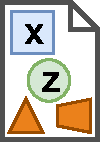
\includegraphics[scale=0.4]{materials/doc-ax-bz-m1-m1p.pdf}};
            
\includegraphics[scale=0.4]{materials/doc-opaque.pdf}};
        \node[left=1pt of docA] {
            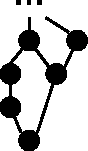
\includegraphics[scale=0.4]{materials/log-sample.pdf}};

        \node[label=above:{\textbf{B}ob}] (B) at (2.1, 1.4) {
            
\includegraphics[scale=0.4]{materials/device.pdf}};
        \node[above right=-22pt and 1pt of B] (docB) {
            %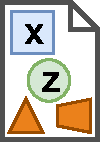
\includegraphics[scale=0.4]{materials/doc-ax-bz-m1-m1p.pdf}};
            
\includegraphics[scale=0.4]{materials/doc-opaque.pdf}};
        \node[right=1pt of docB] {
            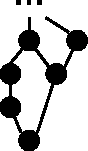
\includegraphics[scale=0.4]{materials/log-sample.pdf}};

        \node[label=below:{\textbf{C}arol}] (D) at (4.1, -0.4) {
            
\includegraphics[scale=0.4]{materials/device.pdf}};
        \node[right=1pt of D] (docD) {
            \includegraphics<3>[scale=0.4]{materials/computations.pdf}%
            %\includegraphics<4>[scale=0.4]{materials/doc-ax-bz-m1-m1p.pdf}};
            \includegraphics<4>[scale=0.4]{materials/doc-opaque.pdf}};
        \node<3,4>[right=1pt of docD] {
            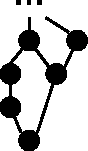
\includegraphics[scale=0.4]{materials/log-sample.pdf}};

        % Network and packets
        \draw[com] (A) to (B);

        \draw<1,3,4>[com] (B) to (D);
        \draw<2 | handout:0>[unicast] (B) -- (D) node[midway]{
            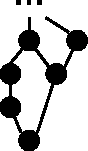
\includegraphics[scale=0.4]{materials/log-sample.pdf}};
    \end{tikzpicture}\end{figure}
    \begin{itemize}
        \item participants \textbf{keep the entire log} for newcomers
        \item<3-> \textbf{newcomers} verify and play the \textbf{entire log}
    \end{itemize}
\end{frame}

\begin{frame}[standout]
    How to reduce overheads of authenticated logs in dynamic groups?
\end{frame}

\begin{frame}{Overview of contributions}
    \begin{figure}\begin{tikzpicture}
        \node at (6.2,0) {}; % Animation fix
        \node at (-2.5,0) {}; % Animation fix
        \ufcircledcounter{-2, 2.1}{4} % Animation frame count

        % Participants and documents
        \node[label=below:{\textbf{A}lice}] (A) at (0, 0) {
            
\includegraphics[scale=0.4]{materials/device.pdf}};
        \node[left=1pt of A] (docA) {
            %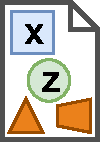
\includegraphics[scale=0.4]{materials/doc-ax-bz-m1-m1p.pdf}};
            
\includegraphics[scale=0.4]{materials/doc-opaque.pdf}};
        \node[left=1pt of docA] {
            \includegraphics<1>[scale=0.4]{materials/log-sample.pdf}
            \includegraphics<2->[scale=0.4]{materials/pruned-log.pdf}
        };

        \node[label=above:{\textbf{B}ob}] (B) at (2.1, 1.4) {
            
\includegraphics[scale=0.4]{materials/device.pdf}};
        \node[above right=-22pt and 1pt of B] (docB) {
            %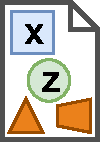
\includegraphics[scale=0.4]{materials/doc-ax-bz-m1-m1p.pdf}};
            
\includegraphics[scale=0.4]{materials/doc-opaque.pdf}};
        \node[right=1pt of docB] {
            \includegraphics<1>[scale=0.4]{materials/log-sample.pdf}
            \includegraphics<2->[scale=0.4]{materials/pruned-log.pdf}
        };

        \node[label=below:{\textbf{C}arol}] (D) at (4.1, -0.4) {
            \includegraphics[scale=0.4]{materials/device.pdf}};
        \node[right=1pt of D] (docD) {
            %\includegraphics<4>[scale=0.4]{materials/doc-ax-bz-m1-m1p.pdf}};
            \includegraphics<4>[scale=0.4]{materials/doc-opaque.pdf}};
        \node[right=1pt of docD] {
            \includegraphics<4>[scale=0.4]{materials/pruned-log.pdf}};

        % Network and packets
        \draw[com] (A) to (B);

        \draw<1,2,4>[com] (B) to (D);
        \draw<3>[unicast] (B) -- (D) node[midway] (joining) {
            %\includegraphics[scale=0.3]{materials/doc-ax-bz-m1-m1p.pdf}};
            \includegraphics[scale=0.3]{materials/doc-opaque.pdf}};

        \node<3>[below=-5pt of joining] {
            \includegraphics[scale=0.3]{materials/pruned-log.pdf}};
    \end{tikzpicture}\end{figure}
    \begin{itemize}
        \item participants \textbf{prune their log}
        \item<3-> newcomers \textbf{retrieve a document and its pruned log}
        \begin{enumerate}
            \item<3-> verify the \textbf{consistency} of the pruned log
            \item<3-> authenticate the document using the pruned log
        \end{enumerate}
    \end{itemize}
\end{frame}

\begin{frame}[standout]
    How to prune a log without threatening convergence?
\end{frame}

\begin{frame}{Pruning issue}
    \begin{columns}
        \begin{column}{0.5\textwidth}
            \begin{figure}\begin{utikzhbgraph}
                \ufcircledcounter{-1.5, 0.5}{2} % Animation frame count
                \node[label=right:{\textbf{A}lice}] at (-0.5, 0.5) {
                    \includegraphics[scale=0.15]{materials/eye.pdf}};
                \only<2>{\transparent{0.4}}
                \node (prefix) at (0, 0) {$\ldots$};
                \uevent{b4}{0,-1}{$b_4$}
                \uevent{a7}{0,-2.3}{$a_7$}
                \only<2>{\transparent{1}}
                \uevent{b5}{0,-3.6}{$b_5$}
                \only<2>{\transparent{0.4}}
                \uhb{prefix}{b4}
                \uhb{b4}{a7}
                \uhb{a7}{b5}
            \end{utikzhbgraph}\end{figure}
        \end{column}
        \begin{column}{0.5\textwidth}
            \begin{figure}\begin{utikzhbgraph}
                \node[label=right:{\textbf{C}arol}] (carol) at (-0.5, 0.5) {
                    \includegraphics[scale=0.15]{materials/eye.pdf}};
                \node (prefix) at (0, 0) {$\ldots$};
                \uevent{b4}{0,-1}{$b_4$}
                \uhb{prefix}{b4}
                \transparent{0}
                \only<2>{\transparent{1}}
                \uevent{c1}{1,-2}{$c_1$}
                \uhb{b4}{c1}
                \node at (0,-3.8) {}; % fix alignement
            \end{utikzhbgraph}\end{figure}
        \end{column}
    \end{columns}
    \begin{itemize}
        \item operations \textbf{cannot be arbitrarily dropped}
        \begin{itemize}
            \item operations are required to verify a given operation
            %\item Only operations that are not involved in verification of future operations can be dropped
        \end{itemize}
        \item concurrency plays an important role
    \end{itemize}
\end{frame}

\begin{frame}{Stability}
    \begin{definition}
        An operation is stable once it is no longer possible to accept a concurrent operation to it.
    \end{definition}
    \begin{itemize}
        \item primitive to define which operations can be dropped
        \begin{itemize}
            \item stable part can be pruned
        \end{itemize}
        \item necessity of \textbf{limiting concurrencies}
    \end{itemize}
\end{frame}

\begin{frame}{Consistency models and Causal consistency}
    \begin{columns}
        \begin{column}{0.5\textwidth}
            \begin{figure}\begin{utikzhbgraph}
                \uevent{a1}{0,0}{$a_{1}$}
                \uevent{a2}{1.7,0.7}{$a_{2}$}
                \uevent{b1}{1.7,-0.7}{$b_{1}$}
                \uevent{b2}{3.4,0}{$b_{2}$}
                \uhb{a1}{a2}
                \uhb{a1}{b1}
                \uhb{a2}{b2}
                \uhb{b1}{b2}
            \end{utikzhbgraph}\end{figure}
            {\centering
            Causal consistent log
            \par}
        \end{column}
        \begin{column}{0.5\textwidth}
            \begin{figure}\begin{utikzhbgraph}
                \uevent{a1}{0,0}{$a_{1}$}
                \uevent{m1}{1.7,0.7}{\color{red}$m_{1}$}
                \uevent{m1p}{1.7,-0.7}{\color{red}$m_1'$}
                \uevent{b1}{3.4,0}{$b_{1}$}
                \uhb{a1}{m1}
                \uhb{a1}{m1p}
                \uhb{m1}{b1}
                \uhb{m1p}{b1}
            \end{utikzhbgraph}\end{figure}
            {\centering
            Non causal consistent log
            \par}
        \end{column}
    \end{columns}
    \vspace{0.5em}
    \begin{itemize}
        \item logs respect a \textbf{consistency model}
        \begin{itemize}
            \item how operations can be related
        \end{itemize}
        \item Causal consistency
        \begin{itemize}
            \item Participants \textbf{linearly order} their operations
        \end{itemize}
    \end{itemize}
\end{frame}

\begin{frame}{Causal Stability\footfullcite{baquero_making_2014}}
    \begin{figure}\begin{utikzhbgraph}
        \node[label=right:{\textbf{B}ob}] at (-0.2, 1.6) {
            \includegraphics[scale=0.15]{materials/eye.pdf}};
        \node[label=right:{group = $\left\{A, B\right\}$}] at (1.4, 1.6) {};
        \node (prefix) at (0, 0) {$\ldots$};
        \uevent{a5}{2,0}{$a_5$}
        \uevent{a6}{4,0.7}{$a_6$}
        \uevent{b3}{4,-0.7}{$b_3$}
        \uevent{b4}{6,0}{$b_4$}
        \uhb{prefix}{a5}
        \uhb{a5}{a6}
        \uhb{a5}{b3}
        \uhb{a6}{b4}
        \uhb{b3}{b4}
        \ulabelled{prefix}{cs}
        \ulabelled{a5}{cs}
        \ulabelled{a6}{cs}
    \end{utikzhbgraph}\end{figure}
    \begin{definition}
        An operation is \emph{causally stable} (cs) once all participants of the group have observed it.
    \end{definition}
    \vspace{1em}
\end{frame}

\begin{frame}{Limitations of Causal Stability}
    \begin{figure}
        \begin{utikzhbgraph}
            \ufcircledcounter{-1.2, 1.6}{3}
            \node<1,3>[label=right:{\textbf{B}ob}] at (-0.2, 1.6) {
                \includegraphics[scale=0.15]{materials/eye.pdf}};
            \node<2>[label=right:{\color{red}\textbf{A}lice}] at (-0.2, 1.6) {
                \includegraphics[scale=0.15]{materials/eye.pdf}};
            \node<1,2>[label=right:{group = $\left\{A, B\right\}$}] at (1.4, 1.6) {};
            \node<3>[label=right:{\color{red}group = ?}] at (1.4, 1.6) {};

            \node (prefix) at (0, 0) {$\ldots$};
            \uevent{a5}{2,0}{$a_5$}
            \uevent{a6}{4,0.7}{$a_6$}
            \uevent{b3}{4,-0.7}{$b_3$}
            \uevent{b4}{6,0}{$b_4$}
            \uhb{prefix}{a5}
            \uhb{a5}{a6}
            \uhb{a5}{b3}
            \uhb{a6}{b4}
            \uhb{b3}{b4}
            \only<1,2>{
                \ulabelled{prefix}{cs}
                \ulabelled{a5}{cs}
                \ulabelled{a6}{cs}
            }
            \only<2>{
                \ulabelled{b3}{cs}
                \ulabelled{b4}{cs}
            }
            \only<1,2>{\transparent{0}}
                \uevent{c1}{6,-1.4}{$c_1$}
                \uhb{b3}{c1}
        \end{utikzhbgraph}
    \end{figure}
    \begin{alertblock}{Issues}
        \begin{itemize}
            \only<1>{\transparent{0}}
            \item convergent logs do not imply \textbf{convergent stability}
            \only<2>{\transparent{0}}
            \item does not fit \textbf{dynamic groups}
            %\item<3-> malicious participants can issue non-linear operations which are \textbf{concurrent to causally stable} operations
        \end{itemize}
    \end{alertblock}
\end{frame}

\begin{frame}{Membership tracking}
    \begin{figure}\begin{utikzhbgraph}
        \node (prefix) at (-2,0) {$\ldots$};
        \uevent{a5}{0, 0}{$a_5$}
        \uparticipants{a5}{below left}{A, B}
        \uhb{prefix}{a5}

        \uevent{a6}{2, 0.8}{$a_6$}
        \uparticipants{a6}{above left}{A, B}
        \uhb{a5}{a6}

        \uevent{b3}{2,-0.8}{$b_3$}
        \uparticipants{b3}{below left}{A, B, {\color{red}C}}
        \uhb{a5}{b3}

        \uevent{b4}{4, 0}{$b_4$}
        \uparticipants{b4}{below right}{A, B, C}
        \uhb{a6}{b4}
        \uhb{b3}{b4}
    \end{utikzhbgraph}\end{figure}
    \begin{itemize}
        \item Operations embed a list of the group members
        \item Dependencies of an operation must include its author
    \end{itemize}
\end{frame}

\begin{frame}{Contribution: Provable causal stability}
    \begin{figure}\begin{utikzhbgraph}
        \ufcircledcounter{-1.7, 1.7}{4}

        \node (prefix) at (-1.5,0) {$\ldots$};
        \uevent{a5}{0, 0}{$a_5$}
        \uparticipants{a5}{above left}{A, B}
        \uhb{prefix}{a5}

        \uevent{a6}{2, 0.8}{$a_6$}
        \uparticipants{a6}{above left}{A, B}
        \uhb{a5}{a6}

        \only<1>{\transparent{0}}
            \uevent{b3}{2,-0.8}{$b_3$}
            \uparticipants{b3}{below left}{A, B, {\color{red} C}}
            \uhb{a5}{b3}
            \ulabelled{a5}{\only<2>{\textbf{pcs}}\only<3->{pcs}}
        \only<2>{\transparent{0}}
            \uevent{b4}{4, 0}{$b_4$}
            \uparticipants{b4}{above right}{A, B,C}
            \uhb{a6}{b4}
            \uhb{b3}{b4}
        \only<3>{\transparent{0}}
            \uevent{c1}{6, 0}{$c_1$}
            \uparticipants{c1}{above right}{A, B,C}
            \uhb{b4}{c1}
            \ulabelled{a6}{\textbf{pcs}}
    \end{utikzhbgraph}\end{figure}
    \vspace{-1.1em}
    \begin{definition}
        An operation is provably causally stable (pcs) once all required observers have provably observed it.
    \end{definition}

    required observers =\vspace{-0.5em}
    \begin{itemize}
        \item[+] participants at the moment of generation
        \item[+] participants concurrently invited
    \end{itemize}
\end{frame}

\begin{frame}{Malicious participants and causal consistency}
    \begin{figure}\begin{utikzhbgraph}
        \node (prefix) at (-1.7,0) {$\ldots$};
        \uevent{a3}{0,0}{$a_3$}
        \uevent{m1p}{1.7,0.7}{\color{red}$m_1'$}
        \uevent{m1}{1.7,-0.7}{\color{red}$m_1$}
        \uevent{b2}{3.4,-0.7}{$b_2$}
        \uevent{a4}{3.4,0.7}{$a_4$}
        \uhb{prefix}{a3}
        \uhb{a3}{m1}
        \uhb{a3}{m1p}
        \uhb{m1p}{a4}
        \uhb{m1}{b2}
    \end{utikzhbgraph}\end{figure}
    \begin{itemize}
        \item Malicious participants can issue \textbf{non-linear operations}
        \begin{itemize}
            \item Causal consistency is not achievable
        \end{itemize}
    \end{itemize}
\end{frame}

\begin{frame}{\acl{VFJC} consistency\footfullcite{mahajan_cac_2011}}
    \begin{columns}
        \begin{column}{0.5\textwidth}
            \begin{figure}\begin{utikzhbgraph}
                \ufcircledcounter{-0.2, 1.6}{3} % Animation frame count
                \node[label=right:{\textbf{A}lice}] at (0.8, 1.6) {
                    \includegraphics[scale=0.15]{materials/eye.pdf}};

                \uevent{a3}{0,0}{$a_3$}
                \uevent{m1p}{1.5,0.7}{\only<2>{\color{red}}$m_1'$}
                \uhb{a3}{m1p}
                \uevent{a4}{3,0.7}{$a_4$}
                \uhb{m1p}{a4}

                \only<1>{\transparent{0}}
                \uevent{m1}{1.5,-0.7}{\only<2>{\color{red}}$m_1$}
                \uhb{a3}{m1}

                \only<2>{\transparent{0}}
                \uevent{b2}{3,-0.7}{$b_2$}
                \uhb{m1}{b2}
            \end{utikzhbgraph}\end{figure}
            {\centering
            \only<2>{\color{red}non }\acs{VFJC}-consistent
            \par}
        \end{column}
        \begin{column}{0.5\textwidth}
            \begin{figure}\begin{utikzhbgraph}
                \node[label=right:{\textbf{B}ob}] at (0.8, 1.6) {
                    \includegraphics[scale=0.15]{materials/eye.pdf}};

                \uevent{a3}{0,0}{$a_3$}
                \uevent{m1}{1.5,-0.7}{$m_1$}
                \uevent{b2}{3,-0.7}{$b_2$}
                \uhb{a3}{m1}
                \uhb{m1}{b2}
            \end{utikzhbgraph}\end{figure}
            {\centering
            \acs{VFJC}-consistent
            \par}
        \end{column}
    \end{columns}
    \begin{itemize}
        \item honest participants linearly order their operations
        \item operations \textbf{cannot directly depend on non-linear} ones
    \end{itemize}
\end{frame}

\begin{frame}{\acs{VFJC} consistency}
    \begin{figure}\begin{utikzhbgraph}
        \node[label=right:{\textbf{A}lice}] at (-1.7, 1.6) {
            \includegraphics[scale=0.15]{materials/eye.pdf}};
        \node[label=right:{group $ \subseteq \left\{A, B, M\right\}$}] at (0, 1.6) {};

        \node[] (prefix) at (-1.7, 0) {$\ldots$};
        \uevent{a3}{0,0}{$a_3$}
        \uhb{prefix}{a3}
        \uevent{m1p}{1.7,0.7}{\color{red}$m_1'$}
        \uhb{a3}{m1p}
        \uevent{a4}{3.4,0.7}{$a_4$}
        \uhb{m1p}{a4}

        \uevent{m1}{1.7,-0.7}{\color{red}$m_1$}
        \uhb{a3}{m1}

        \uevent{b2}{3.4,-0.7}{$b_2$}
        \uhb{m1}{b2}

        \uevent{a5}{5.1,0}{$a_5$}
        \uhb{a4}{a5}
        \uhb{b2}{a5}

        \ulabelled{prefix}{pcs}
        \ulabelled{a3}{pcs}
        \ulabelled{m1}{\textbf{pcs}}
        \uparticipants{a5}{above right}{A, B}
    \end{utikzhbgraph}\end{figure}
    \begin{itemize}
        \item \textbf{impossibility of} honestly accepting concurrent operations which are \textbf{non-linear with a provably causally stable} operation
    \end{itemize}
\end{frame}

\begin{frame}{Contribution: \acs{VFJC} Stability}
    \begin{figure}\begin{utikzhbgraph}
        \node[label=right:{\textbf{A}lice}] at (-1.7, 1.6) {
            \includegraphics[scale=0.15]{materials/eye.pdf}};
        \node[label=right:{group $\subseteq \left\{A, B, M\right\}$}] at (0, 1.6) {};

        \node[] (prefix) at (-1.7, 0) {$\ldots$};
        \uevent{a3}{0,0}{$a_3$}
        \uhb{prefix}{a3}
        \uevent{m1p}{1.7,0.7}{\color{red}$m_1'$}
        \uhb{a3}{m1p}
        \uevent{a4}{3.4,0.7}{$a_4$}
        \uhb{m1p}{a4}

        \uevent{m1}{1.7,-0.7}{\color{red}$m_1$}
        \uhb{a3}{m1}

        \uevent{b2}{3.4,-0.7}{$b_2$}
        \uhb{m1}{b2}

        \uevent{a5}{5.1,0}{$a_5$}
        \uhb{a4}{a5}
        \uhb{b2}{a5}

        \uevent{b3}{6.9,0}{$b_3$}
        \uhb{a5}{b3}

        \ulabelled{prefix}{vfjcs}
        \ulabelled{a3}{vfjcs}
        \ulabelled{m1}{vfjcs}
        \ulabelled{m1p}{pcs}
        \ulabelled{a4}{pcs}
        \ulabelled{b2}{vfjcs}
        \ulabelled{a5}{pcs}
        \uparticipants{a5}{above right}{A, B}
    \end{utikzhbgraph}\end{figure}
    \begin{definition}
        An operation is \acs{VFJC}-stable (vfjcs) once all required observers have a provably causally stable operation which depends on.
    \end{definition}
    \begin{itemize}
        \item \acs{VFJC} stability $\implies$ provable causal stability
    \end{itemize}
\end{frame}

\begin{frame}{Stability}
    \begin{tabular}{r| c c c c}
        Stability & CS & \textbf{PCS} & \textbf{VFJCS} & \textbf{VFJCS} \\ \hline
        Consistency model & Causal & $\sim$ Causal & \acs{VFJC} & \textbf{SVFJC} \\
        Group membership & Static & Dynamic & Static & Dynamic \\
        environment & Honest & Honest & Malicious & Malicious \\
    \end{tabular}
    \begin{description}
    \item[CS:] Causal Stability
    \item[PCS:] Provable Causal Stability
    \item[VFJC:] \acl{VFJC}
    \item[VFJCS:] \acl{VFJC} Stability
    \item[SVFJC:] Stabilizable \acl{VFJC}
    \end{description}
\end{frame}

\begin{frame}{Conclusions}
    \begin{block}{Contributions}
        \begin{itemize}
            \item adaptation of \textbf{Causal Stability for dynamic groups}
            \item definition of \textbf{\acs{VFJC} Stability}
            \item Stabilizable \ac{VFJC} (not covered here)
            \item document \textbf{authentication based on a pruned log}
        \end{itemize}
    \end{block}
    \begin{block}{Perspectives}
        \begin{itemize}
            \item exploring sub-group log pruning
            \item \acs{VFJC} Stability as building block of \textbf{asynchronous Byzantine consensus}
        \end{itemize}
    \end{block}
\end{frame}

\begin{frame}
    \vspace{1em}
    \printbibliography%
    \begin{center}\ccby\hspace{3pt}4.0\end{center}
\end{frame}

% Backup slides
% -------------

\begin{frame}[standout]
    How to authenticate an untrusted snapshot?
\end{frame}

\begin{frame}{Overview of document authentication}
    \begin{columns}
        \begin{column}{0.75\textwidth}
            \begin{figure}\begin{utikzhbgraph}
                \uevent{b70}{0,0.8}{$b_{70}$}
                \uevent{m2}{1.5,0.8}{$m_2$}
                \uhb{b70}{m2}
                \uevent{a82}{3,0.8}{$a_{82}$}
                \uhb{m2}{a82}
                \uevent{m2p}{0,-0.8}{$m_2'$}
                \uevent{b71}{1.5,-0.8}{$b_{71}$}
                \uhb{b70}{b71}
                \uhb{m2p}{b71}
                \uevent{b72}{4.5,-0.8}{$b_{72}$}
                \uembedded{b72}{below left}{invite Dave}
                \uembedded{b72}{below right}{
                    \includegraphics[scale=0.15]{materials/fingerprint.pdf}}
                \uhb{a82}{b72}
                \uhb{b71}{b72}
                \uevent{a83}{6,-0.8}{$a_{83}$}
                \uhb{b72}{a83}

                \draw[thick,dotted] ($(b72.south west)+(-0.3,-0.3)$) rectangle ($(a83.north east)+(0.3,0.3)$) node[above,xshift=-1.3cm]{trusted set};
            \end{utikzhbgraph}\end{figure}
        \end{column}
        \begin{column}{0.25\textwidth}
            \begin{utikzhbgraph}
                \node (snapshot) at (0,0) {
                    \includegraphics[scale=0.8]{materials/untrusted-document.pdf}};
                \node[below=10pt of snapshot,label=below:{computed}] {
                    \includegraphics[scale=0.15]{materials/fingerprint.pdf}};
            \end{utikzhbgraph}
        \end{column}
    \end{columns}
    \begin{itemize}
        \item participants embed a \textbf{document fingerprint in invitations}
        \begin{itemize}
            \item participants verify fingerprints
        \end{itemize}
        \item \textbf{computed} fingerprint = \textbf{embedded} fingerprint\\$\implies$ \textbf{document considered authentic}
        \item a newcomer trusts a \textbf{fingerprint verified by her trusted set}
    \end{itemize}
\end{frame}
\end{document}
